\documentclass[12pt,a4paper]{article}

\usepackage[utf8]{inputenc}
\usepackage[T1]{fontenc}
\usepackage{textcomp}
\usepackage[spanish,es-tabla]{babel}
\usepackage{lmodern}
\usepackage{geometry}
\usepackage{setspace}
\usepackage{graphicx}
\usepackage{float}
\usepackage{booktabs}
\usepackage{tabularx}
\usepackage{longtable}
\usepackage{array}
\usepackage{amsmath}
\usepackage{enumitem}
\usepackage{xcolor}
\usepackage{listings}
\usepackage{caption}
\usepackage{subcaption}
\usepackage{pdflscape}
\usepackage{hyperref}
\usepackage{fancyhdr}

\geometry{margin=2.5cm}
\onehalfspacing
\setlength{\parskip}{0.45em}
\setlength{\parindent}{0pt}
\setlist[itemize]{leftmargin=1.2cm}
\setlist[enumerate]{leftmargin=1.2cm}

\definecolor{codegray}{RGB}{245,245,245}
\definecolor{linkblue}{RGB}{22,82,150}

\hypersetup{
    colorlinks=true,
    linkcolor=linkblue,
    urlcolor=linkblue,
    citecolor=linkblue,
    pdftitle={Informe Final Spark HDFS Arbitrios MDJM},
    pdfauthor={Grupo CC531}
}

\pagestyle{fancy}
\fancyhf{}
\lhead{CC531 A - An\'alisis en Macrodatos}
\rhead{Examen Final}
\cfoot{\thepage}

\lstdefinelanguage{scala}{
  morekeywords={abstract,case,catch,class,def,do,else,extends,false,final,finally,for,forSome,if,implicit,import,lazy,match,new,null,object,override,package,private,protected,return,sealed,super,this,throw,trait,true,try,type,val,var,while,with,yield},
  sensitive=true,
  morecomment=[l]{//},
  morecomment=[s]{/*}{*/},
  morestring=[b]"
}

\lstdefinelanguage{bash}{
  morekeywords={cd,make,time,hdfs,spark-submit},
  sensitive=true,
  morecomment=[l]{\#},
  morestring=[b]"
}

\lstset{
    basicstyle=\ttfamily\footnotesize,
    backgroundcolor=\color{codegray},
    breaklines=true,
    frame=single,
    framerule=0.2pt,
    columns=fullflexible,
    keepspaces=true,
    showstringspaces=false,
    tabsize=2
}

\newcommand{\projecttitle}{Implementaci\'on y evaluaci\'on de un cl\'uster Spark con HDFS para el an\'alisis de arbitrios municipales de Jes\'us Mar\'ia}
\newcommand{\datasetname}{Emisi\'on de arbitrios municipales de la Municipalidad Distrital de Jes\'us Mar\'ia}

\begin{document}

\begin{titlepage}
    \centering
    {\Large Universidad Nacional de Ingenier\'ia \par}
    \vspace{0.2cm}
    {\large Facultad de Ciencias \par}
    \vspace{0.1cm}
    {\large Escuela Profesional de Ciencia de la Computaci\'on \par}
    \vspace{1.2cm}

    {\Large \textbf{CC531 A - An\'alisis en Macrodatos 2026-I}\par}
    \vspace{0.4cm}
    {\large Examen Final - Parte 2\par}
    \vspace{1.6cm}

    {\Huge \textbf{\projecttitle}\par}
    \vspace{1.0cm}
    {\Large Dataset: \datasetname\par}

    \vfill

    \begin{tabular}{rl}
        \textbf{Integrante 1:} & Nombre Apellido - Codigo \\
        \textbf{Integrante 2:} & Nombre Apellido - Codigo \\
        \textbf{Integrante 3:} & Nombre Apellido - Codigo \\
        \textbf{Docente:} & Nombre del docente \\
        \textbf{Fecha:} & 8 de julio de 2026 \\
    \end{tabular}

    \vfill

    \textbf{Entregables asociados:} informe, c\'odigo Scala, salidas JSON, capturas de ejecuci\'on mononodo y multimodo, gr\'aficos de p\'erdida y dataset utilizado.
\end{titlepage}

\tableofcontents
\newpage

\section{Resumen}

El presente informe documenta la implementacion de un cluster Apache Spark con HDFS en modo multimodo y su uso para procesar un dataset de la Plataforma Nacional de Datos Abiertos relacionado con economia y finanzas municipales. El caso de estudio corresponde a la emision de arbitrios municipales de la Municipalidad Distrital de Jesus Maria, con 222\,874 registros del periodo 2023--2025.

El trabajo cubre el ciclo completo solicitado en el examen: carga desde HDFS, generacion de dos tablas JSON, dos consultas Spark SQL, dos modelos de regresion con campos decimales, dos modelos de clasificacion, metricas comparativas entre una ejecucion de un solo nodo y una ejecucion distribuida, graficos de perdida de entrenamiento y evidencias visuales del uso de recursos por nodo.

La arquitectura distribuida quedo conformada por un nodo maestro y dos nodos esclavos sobre maquinas virtuales Ubuntu. Aunque la ejecucion multimodo finalizo correctamente, el tiempo total fue mayor que el obtenido en mononodo. Este resultado es coherente con el tamano moderado del dataset y con el costo adicional de YARN, HDFS, transferencia de bloques, shuffle distribuido y virtualizacion.

\section{Dataset utilizado}
\label{sec:dataset}

\subsection{Fuente y descripcion}

Se utilizo el dataset \textit{\datasetname}, obtenido desde la Plataforma Nacional de Datos Abiertos del Peru (PNDA) y publicado por la Municipalidad Distrital de Jesus Maria - Lima. En la ficha oficial, el conjunto aparece dentro de la categoria Economia y Finanzas y asociado a Dataton 2025. El dataset contiene informacion de emision de arbitrios municipales por predio, contribuyente y periodo, incluyendo montos por parques y jardines, serenazgo, residuos solidos, barrido de calles y descuentos asociados.

La ficha PNDA registra fecha de lanzamiento 2025-04-24, fecha de modificacion 2025-08-06, licencia Open Data Commons Attribution License y acceso publico. La copia trabajada contiene 222\,874 registros y 18 columnas, con datos para los periodos 2023, 2024 y 2025. El archivo local empleado fue \texttt{data/dataset\_vf\_3.csv}, delimitado por punto y coma. La columna \texttt{FECHA\_CORTE} coincide con la fecha de lanzamiento del dataset para la muestra revisada de 2025.

\subsection{Relacion con economia y finanzas}

El conjunto pertenece al ambito de economia y finanzas municipales porque registra obligaciones tributarias locales asociadas a servicios municipales. Su analisis permite estudiar recaudacion potencial, distribucion de cargas por predio, comportamiento por periodo y diferencias entre tipos de predios.

\subsection{Investigaciones previas y uso del dataset}

No se identificaron, dentro de la informacion local del proyecto, articulos academicos que utilicen exactamente este dataset de arbitrios de Jesus Maria. Por ello, el trabajo se plantea como un analisis reproducible sobre una base publica reciente, orientado a transparencia fiscal y analitica municipal. Como antecedente metodologico se consideran los usos generales de datos abiertos gubernamentales para rendicion de cuentas, fiscalizacion ciudadana y mejora de servicios publicos.

\subsection{Campos principales}

Los campos usados en el procesamiento fueron:

\begin{itemize}
    \item Identificacion: \texttt{COD\_CONTRIBUYENTE}, \texttt{NOM\_CONTRIBUYENTE}, \texttt{COD\_PREDIO}.
    \item Tiempo y ubicacion: \texttt{FECHA\_CORTE}, \texttt{PERIODO}, \texttt{UBIGEO}, \texttt{DEPARTAMENTO}, \texttt{PROVINCIA}, \texttt{DISTRITO}.
    \item Montos decimales: \texttt{MONTO\_PARQUE\_JARDIN}, \texttt{MONTO\_SERENAZGO}, \texttt{MONTO\_RESIDUO\_SOLIDO}, \texttt{MONTO\_BARRIDO\_CALLE}.
    \item Descuentos y topes: \texttt{DESCUENTO\_TOPE\_PARQUE\_JARDIN}, \texttt{DESCUENTO\_TOPE\_SERENAZGO}, \texttt{MONTO\_TOPE\_RESIDUO\_SOLIDO}, \texttt{DESCUENTO\_TOPE\_BARRIO\_CALLE}.
    \item Condominio: \texttt{PORCENTAJE\_CONDOMINIO}, usado para distinguir predios exclusivos y compartidos.
\end{itemize}

\subsection{Limpieza de datos}

El CSV presenta montos con coma como separador de miles, por ejemplo \texttt{1,257.60}. En el ETL se elimino la coma antes de castear a \texttt{Double}, evitando interpretar estos valores como texto. Esta limpieza se implemento en \texttt{ETL.DecimalCols}, aplicada a todas las columnas monetarias y porcentuales.

\section{Implementaci\'on del cl\'uster Spark con HDFS}

\subsection{Arquitectura desplegada}

La arquitectura multimodo implementada se compone de tres maquinas virtuales Ubuntu:

\begin{itemize}
    \item \textbf{master}: ejecuta NameNode de HDFS, ResourceManager de YARN y participa como nodo de computo.
    \item \textbf{slave1}: ejecuta DataNode y NodeManager.
    \item \textbf{slave-base}: ejecuta DataNode y NodeManager.
\end{itemize}

El almacenamiento distribuido se gestiono con HDFS y la ejecucion de Spark se realizo sobre YARN. La entrada principal del proyecto se ubico en \texttt{hdfs:///mdjm/input/dataset\_vf\_3.csv} y la salida completa de verificacion en \texttt{hdfs:///mdjm/output\_3nodes\_verify\_20260707\_2325}.

\subsection{Versiones y recursos}

\begin{table}[H]
    \centering
    \caption{Versiones y configuracion base del entorno.}
    \label{tab:versions}
    \begin{tabularx}{\textwidth}{lX}
        \toprule
        \textbf{Componente} & \textbf{Configuracion verificada} \\
        \midrule
        Hadoop & 3.3.0 \\
        Spark & 3.4.0, Scala 2.12.17 \\
        Gestor de recursos & YARN, Capacity Scheduler \\
        Nodos activos & 3: \texttt{master}, \texttt{slave1}, \texttt{slave-base} \\
        Recursos YARN totales & 8 GB de memoria y 4 vcores \\
        Recursos master & 4 GB, 2 vcores \\
        Recursos por worker & 2 GB, 1 vcore por nodo \\
        Interfaz YARN & \url{http://192.168.1.48:8088} \\
        Interfaz NameNode & \url{http://192.168.1.48:9870} \\
        Spark UI en ejecucion & \url{http://192.168.1.48:4040} \\
        \bottomrule
    \end{tabularx}
\end{table}

\subsection{Pasos principales de implementacion}

Los pasos aplicados fueron:

\begin{enumerate}
    \item Verificar conectividad entre los tres nodos mediante nombres de host \texttt{master}, \texttt{slave1} y \texttt{slave-base}.
    \item Revisar espacio disponible y crear directorios temporales para Spark en cada nodo.
    \item Configurar HDFS con NameNode en el master y DataNodes en los workers.
    \item Configurar YARN con ResourceManager en el master y NodeManagers en los tres nodos.
    \item Instalar y validar Spark en \texttt{/opt/spark}.
    \item Definir variables de entorno: \texttt{SPARK\_HOME}, \texttt{HADOOP\_CONF\_DIR}, \texttt{YARN\_CONF\_DIR} y \texttt{SPARK\_LOCAL\_DIRS}.
    \item Subir el dataset a HDFS y ejecutar el jar \texttt{arbitrios-mdjm.jar} con \texttt{spark-submit --master yarn}.
    \item Monitorear la ejecucion con YARN UI, Spark UI, comandos \texttt{yarn node -list -showDetails} y \texttt{htop}.
\end{enumerate}

\subsection{Pruebas de configuracion y conectividad}

La conectividad entre Hadoop, YARN y Spark se valido desde el nodo maestro. La prueba principal fue consultar YARN con \texttt{yarn node -list -showDetails}, ya que este comando confirma que los tres NodeManagers se comunican con el ResourceManager y reportan estado \texttt{RUNNING}. Esto demuestra que el master reconoce a \texttt{slave1} y \texttt{slave-base} como nodos disponibles para ejecutar contenedores.

Adicionalmente, se revisaron los archivos de configuracion de Hadoop y Spark:

\begin{itemize}
    \item \texttt{workers}: lista los nodos que participan como workers.
    \item \texttt{core-site.xml}: define \texttt{fs.defaultFS} apuntando al NameNode del master.
    \item \texttt{hdfs-site.xml}: configura almacenamiento distribuido y replicacion.
    \item \texttt{yarn-site.xml}: define ResourceManager, NodeManagers, memoria y vcores.
    \item \texttt{spark-env.sh} y \texttt{spark-defaults.conf}: conectan Spark con Hadoop/YARN mediante \texttt{HADOOP\_CONF\_DIR}, \texttt{YARN\_CONF\_DIR} y \texttt{spark.master yarn}.
\end{itemize}

Estas pruebas son importantes porque no basta con instalar Spark en cada maquina; Spark debe leer la configuracion de Hadoop para ubicar HDFS y debe enviar sus aplicaciones a YARN para que los ejecutores se distribuyan entre los nodos.

\subsection{Evidencias visuales de ejecucion}

\begin{figure}[H]
    \centering
    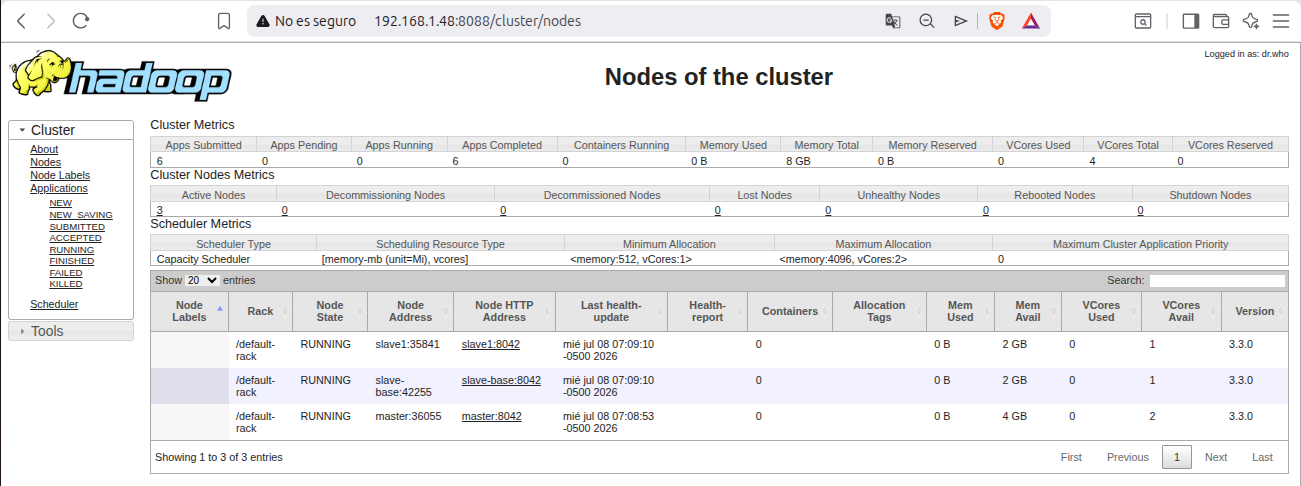
\includegraphics[width=\textwidth]{ImgMultiNodo/Nodes_02_yarn_nodos_cluster_activos.png}
    \caption{Interfaz YARN con los tres nodos activos: \texttt{master}, \texttt{slave1} y \texttt{slave-base}.}
    \label{fig:yarn-nodes}
\end{figure}

\begin{figure}[H]
    \centering
    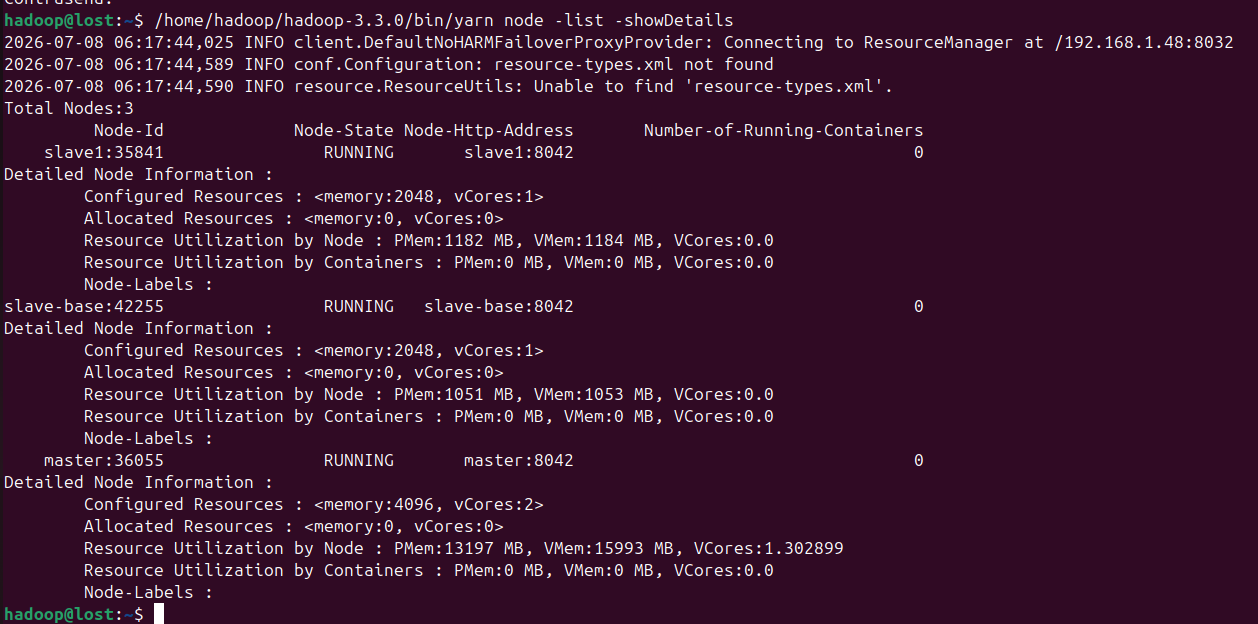
\includegraphics[width=\textwidth]{ImgMultiNodo/VerificarCluster_Los3Activos.png}
    \caption{Verificacion por terminal de los tres nodos activos mediante \texttt{yarn node -list -showDetails}.}
    \label{fig:yarn-terminal-nodes}
\end{figure}

\begin{figure}[H]
    \centering
    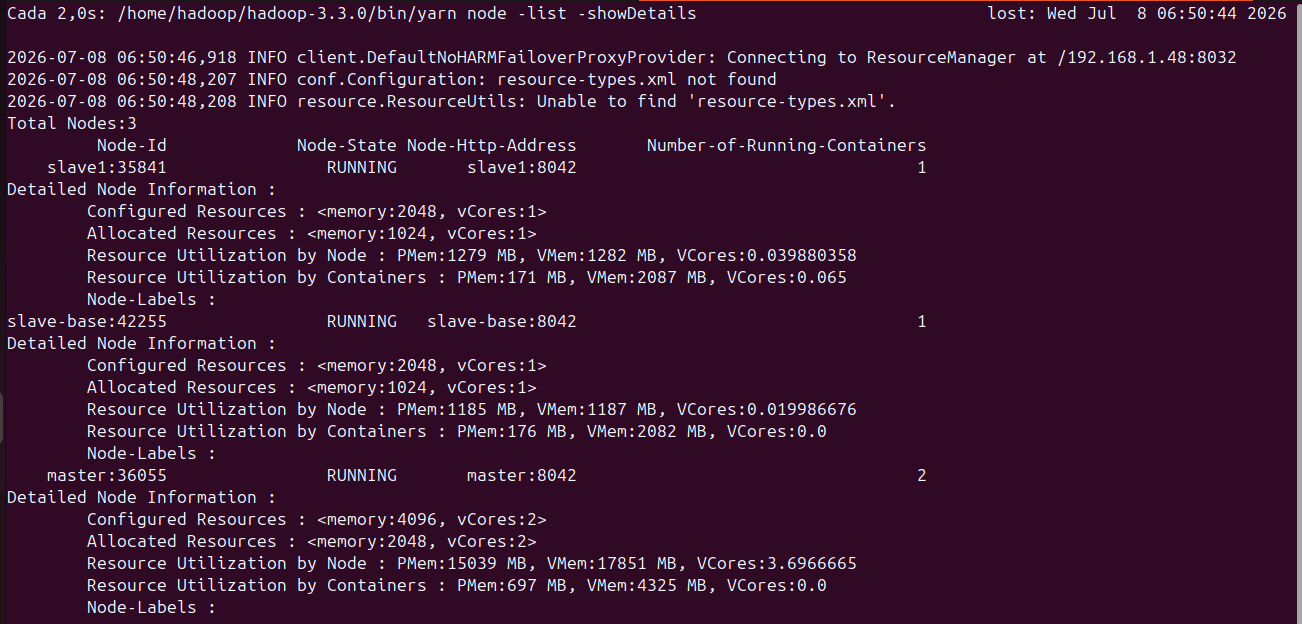
\includegraphics[width=\textwidth]{ImgMultiNodo/yarn_node_showdetails_live.png}
    \caption{Monitoreo por terminal durante la ejecucion distribuida: contenedores activos y recursos asignados por nodo.}
    \label{fig:yarn-live}
\end{figure}

\begin{figure}[H]
    \centering
    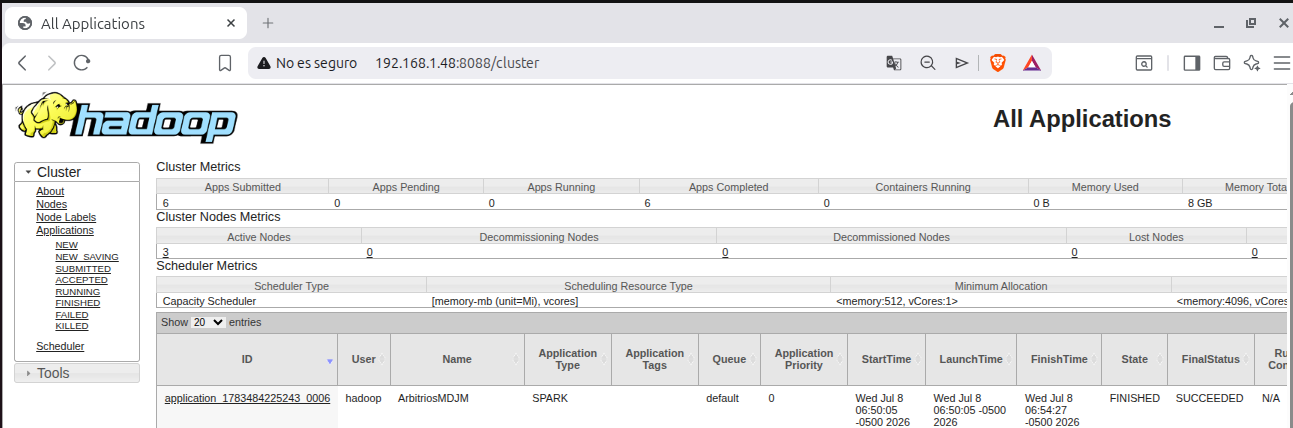
\includegraphics[width=\textwidth]{ImgMultiNodo/cluster_01_yarn_aplicacion_spark_succeeded.png}
    \caption{Aplicacion Spark \texttt{ArbitriosMDJM} finalizada exitosamente en YARN.}
    \label{fig:yarn-succeeded}
\end{figure}

\begin{figure}[H]
    \centering
    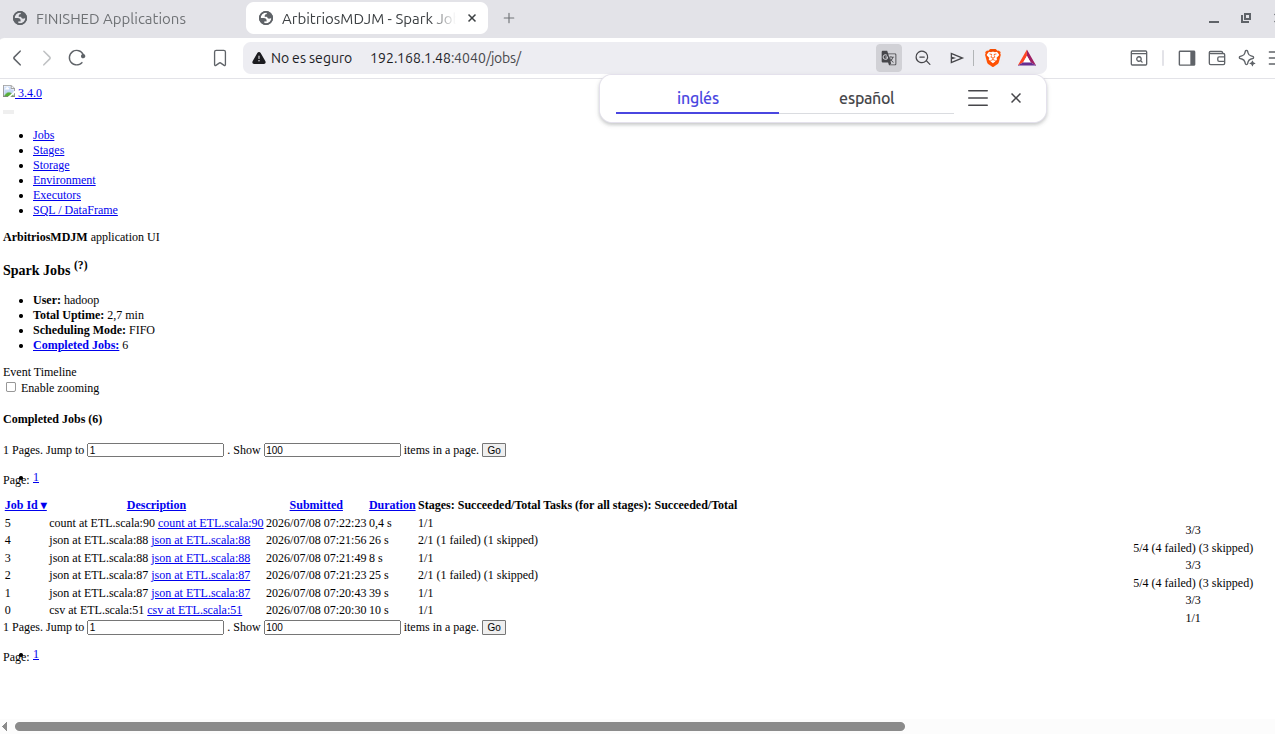
\includegraphics[width=\textwidth]{ImgMultiNodo/SparkUIETL.png}
    \caption{Spark UI durante la etapa ETL, con trabajos completados para lectura, transformacion y escritura en JSON.}
    \label{fig:spark-ui-etl}
\end{figure}

\section{Generaci\'on de tablas JSON y consultas Spark SQL}

\subsection{ETL y tablas generadas}

El ETL lee el CSV desde HDFS o disco local, limpia columnas decimales, castea los campos temporales y genera dos tablas JSON:

\begin{itemize}
    \item \texttt{contribuyentes.json}: dimension de contribuyentes con \texttt{COD\_CONTRIBUYENTE} y \texttt{NOM\_CONTRIBUYENTE}. Se conserva el nombre mas reciente por contribuyente.
    \item \texttt{emisiones.json}: tabla de hechos con granularidad \texttt{(COD\_PREDIO, COD\_CONTRIBUYENTE, PERIODO)}. Esta tabla contiene los montos, descuentos, porcentaje de condominio y ubigeo.
\end{itemize}

La corrida local verifico 222\,874 filas crudas, 47\,175 contribuyentes y 222\,873 emisiones despues de eliminar un duplicado exacto sobre la clave natural de hechos.

\begin{figure}[H]
    \centering
    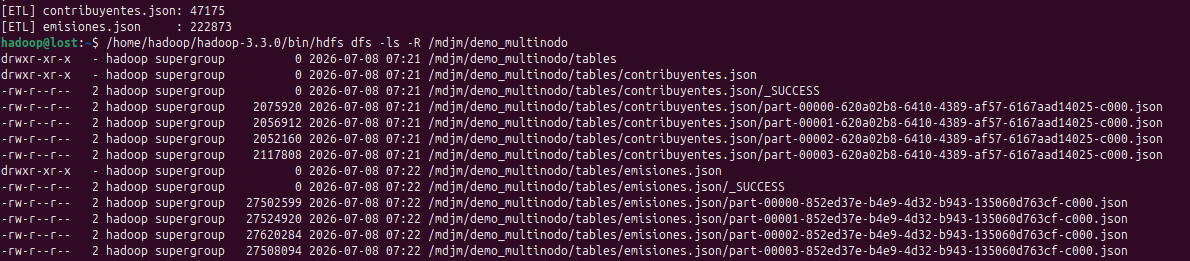
\includegraphics[width=\textwidth]{ImgMultiNodo/json_Contribuyente_emisiones.png}
    \caption{Salidas HDFS generadas por el ETL en \texttt{contribuyentes.json} y \texttt{emisiones.json}.}
    \label{fig:hdfs-tables}
\end{figure}

\subsection{Preguntas respondidas y relacion con el codigo}

La Tabla~\ref{tab:preguntas-consultas} resume, para cada grupo de pregunta solicitado, la consulta analitica que responde, las columnas o caracteristicas empleadas, la solucion implementada, la interpretacion de los resultados y el archivo Scala asociado.

%\begin{longtable}{p{0.12\textwidth}p{0.22\textwidth}p{0.26\textwidth}p{0.25\textwidth}}
\setlength{\emergencystretch}{3em}
\begin{longtable}{
  p{0.12\textwidth}
  p{0.22\textwidth}
  p{0.26\textwidth}
  p{\dimexpr0.40\textwidth-8\tabcolsep\relax}
}
\caption{Preguntas del dataset, solucion aplicada e interpretacion.}

\label{tab:preguntas-consultas}\\

\toprule

\textbf{Item} & \textbf{Pregunta que responde} & \textbf{Columnas/\newline caracteristicas usadas} & \textbf{Solucion e \newline interpretacion} \\

\midrule

\endfirsthead

\toprule

\textbf{Item} & \textbf{Pregunta que responde} & \textbf{Columnas/\newline caracteristicas usadas} & \textbf{Solucion e \newline interpretacion} \\

\midrule

\endhead

ETL y tablas JSON &

¿Como separar el dataset original en estructuras reutilizables sin depender de PostgreSQL? &

\texttt{COD\_CONTRIBUYENTE}, \texttt{NOM\_CONTRIBUYENTE}, \texttt{COD\_PREDIO}, \texttt{PERIODO}, montos, descuentos y \texttt{UBIGEO}. &

Se generan \texttt{contribuyentes.json} y \texttt{emisiones.json}. La primera funciona como dimension y la segunda como tabla de hechos a nivel predio-contribuyente-periodo. Codigo: \texttt{ETL.scala}. \\

\midrule

SQL 1: \texttt{groupBy} + funciones &

¿Cuanto se emitio en total y en promedio por concepto municipal durante cada periodo? &

\texttt{PERIODO}, \texttt{MONTO\_PARQUE\_JARDIN}, \texttt{MONTO\_SERENAZGO}, \texttt{MONTO\_RESIDUO\_SOLIDO}, \texttt{MONTO\_BARRIDO\_CALLE}. &

Se agrupa por periodo y se aplican \texttt{sum}, \texttt{avg}, \texttt{count} y \texttt{round}. Permite comparar la evolucion anual de la emision por concepto. Codigo: \texttt{SqlQueries.query1GroupByPeriodo}. \\

\midrule

SQL 2: vista temporal + \texttt{ORDER BY} &

¿Cuales son los predios exclusivos con mayor monto total neto en 2025? &

\texttt{COD\_PREDIO}, \texttt{COD\_CONTRIBUYENTE}, \texttt{PERIODO}, \texttt{PORCENTAJE\_CONDOMINIO}, montos y descuentos. &

Se crea una vista temporal y se filtra 2025 con condominio 100. Luego se calcula monto neto y se ordena de mayor a menor. Codigo: \texttt{SqlQueries.query2TopPrediosTempView}. \\

\midrule

Regresion MLP &

¿Se puede estimar el monto de serenazgo a partir de variables monetarias y del periodo? &

\texttt{MONTO\_SERENAZGO} como etiqueta; \texttt{PERIODO}, \texttt{PORCENTAJE\_CONDOMINIO}, montos y descuentos como features. &

Se implementa un MLP de regresion con salida lineal y perdida MSE. El menor RMSE frente a SVR indica mejor ajuste global para esta tarea. Codigo: \texttt{MLPRegressor.scala}. \\

\midrule

Regresion SVR &

?Como se comporta una regresion basada en SVM para estimar serenazgo? &

Mismas variables de regresion que MLP para mantener comparabilidad. &

Se implementa SVR lineal con perdida epsilon-insensitiva. Tiene resultados positivos, pero mayor RMSE que MLP. Codigo: \texttt{SVRegressor.scala}. \\

\midrule

Clasificacion Random Forest &

¿Se puede clasificar un predio como exclusivo o compartido usando variables decimales sin fuga de datos? &

\texttt{TIPO\_PREDIO} como etiqueta derivada; se excluye \texttt{PORCENTAJE\_CONDOMINIO} de las features para evitar fuga. &

Random Forest logra el mejor F1-score. Su interpretacion es que los arboles capturan mejor reglas por umbral y relaciones no lineales. Codigo: \texttt{RFAndMLPClassification.scala}. \\

\midrule

Clasificacion MLP &

¿Que desempeno tiene una red neuronal para clasificar tipo de predio frente a Random Forest? &

Mismas variables de clasificacion que Random Forest. &

MLPClassifier funciona, pero obtiene menor F1-score que Random Forest, por lo que requiere mayor ajuste. Codigo: \texttt{RFAndMLPClassification.scala}. \\

\bottomrule

\end{longtable}

\subsection{Consulta 1: recaudacion por periodo}

\textbf{Pregunta de an\'alisis:} \textquestiondown Cu\'anto se emiti\'o en total y en promedio por concepto municipal durante cada periodo?

La primera consulta utiliza la API DataFrame de Spark con \texttt{groupBy("PERIODO")} y funciones de \texttt{org.apache.spark.sql.functions}: \texttt{sum}, \texttt{avg}, \texttt{round} y \texttt{count}. El resultado permite comparar la evolucion anual de los conceptos de parques y jardines, serenazgo, residuos solidos y barrido de calles.

\begin{table}[H]
    \centering
    \caption{Resultado de la consulta 1: totales y promedios por periodo.}
    \label{tab:query1}
    \resizebox{\textwidth}{!}{%
    \begin{tabular}{rrrrrrrrr}
        \toprule
        \textbf{Periodo} & \textbf{Total parques} & \textbf{Prom. parques} & \textbf{Total serenazgo} & \textbf{Prom. serenazgo} & \textbf{Total residuos} & \textbf{Prom. residuos} & \textbf{Total barrido} & \textbf{Emisiones} \\
        \midrule
        2023 & 11\,744\,689.56 & 168.07 & 24\,439\,219.92 & 349.73 & 9\,683\,019.72 & 138.57 & 2\,643\,129.06 & 69\,880 \\
        2024 & 12\,587\,472.36 & 170.15 & 26\,232\,272.82 & 354.59 & 8\,767\,155.37 & 118.51 & 2\,820\,661.03 & 73\,980 \\
        2025 & 11\,919\,521.07 & 150.86 & 27\,835\,182.83 & 352.29 & 9\,816\,547.57 & 124.24 & 3\,314\,446.63 & 79\,013 \\
        \bottomrule
    \end{tabular}}
\end{table}


\subsection{Consulta 2: top de predios exclusivos 2025}

\textbf{Pregunta de an\'alisis:} \textquestiondown Cu\'ales son los predios de propiedad exclusiva con mayor monto total neto en 2025?

La segunda consulta registra \texttt{emisiones} como vista temporal y ejecuta SQL con filtros \texttt{WHERE PERIODO = 2025} y \texttt{PORCENTAJE\_CONDOMINIO = 100}, calculando el monto total neto y ordenando de forma descendente con \texttt{ORDER BY}. La salida final se limita a los 20 predios principales.

\begin{table}[H]
    \centering
    \caption{Primeros 10 registros del top 20 de predios exclusivos 2025 por monto total neto.}
    \label{tab:query2}
    \resizebox{\textwidth}{!}{%
    \begin{tabular}{llrr}
        \toprule
        \textbf{COD\_PREDIO} & \textbf{COD\_CONTRIBUYENTE} & \textbf{Periodo} & \textbf{Monto neto} \\
        \midrule
        6ffc4409...fd253b6 & 38548de4...f0788ef56 & 2025 & 284\,967.96 \\
        6caa5d8c...e4b6ca27 & c55edd28...8d6d48b72 & 2025 & 238\,877.52 \\
        651ead64...87fc39e1 & 38548de4...f0788ef56 & 2025 & 203\,219.88 \\
        48f6cd74...7967f794 & 39ed9d90...665df386 & 2025 & 193\,386.84 \\
        a95619fe...e16a14092 & 39ed9d90...665df386 & 2025 & 190\,837.20 \\
        08bd0c59...51e9d156 & 4539797a...4397e739 & 2025 & 187\,427.40 \\
        ba03f0a6...ebda7ec0 & 38548de4...f0788ef56 & 2025 & 178\,622.28 \\
        2c210356...c38f58fb & 549998ab...3c379ed & 2025 & 175\,102.68 \\
        1d97b755...abb9073e & 55351ada...0abb9073e & 2025 & 148\,005.60 \\
        3db57089...a933474 & d5c17c98...ceb885ed & 2025 & 144\,528.84 \\
        \bottomrule
    \end{tabular}}
\end{table}


\begin{figure}[H]
    \centering
    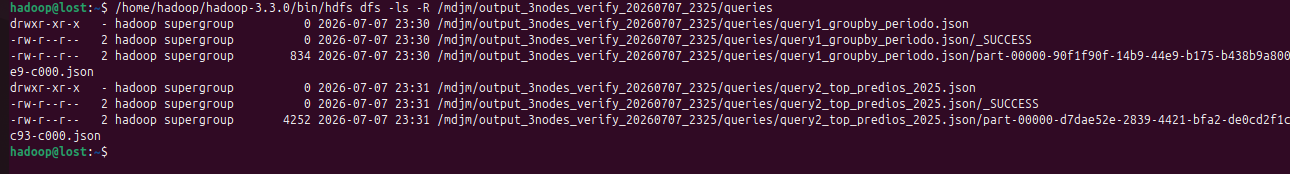
\includegraphics[width=\textwidth]{ImgMultiNodo/json_query_1_2.png}
    \caption{Directorios HDFS generados para las dos consultas Spark SQL.}
    \label{fig:hdfs-queries}
\end{figure}

\begin{figure}[H]
    \centering
    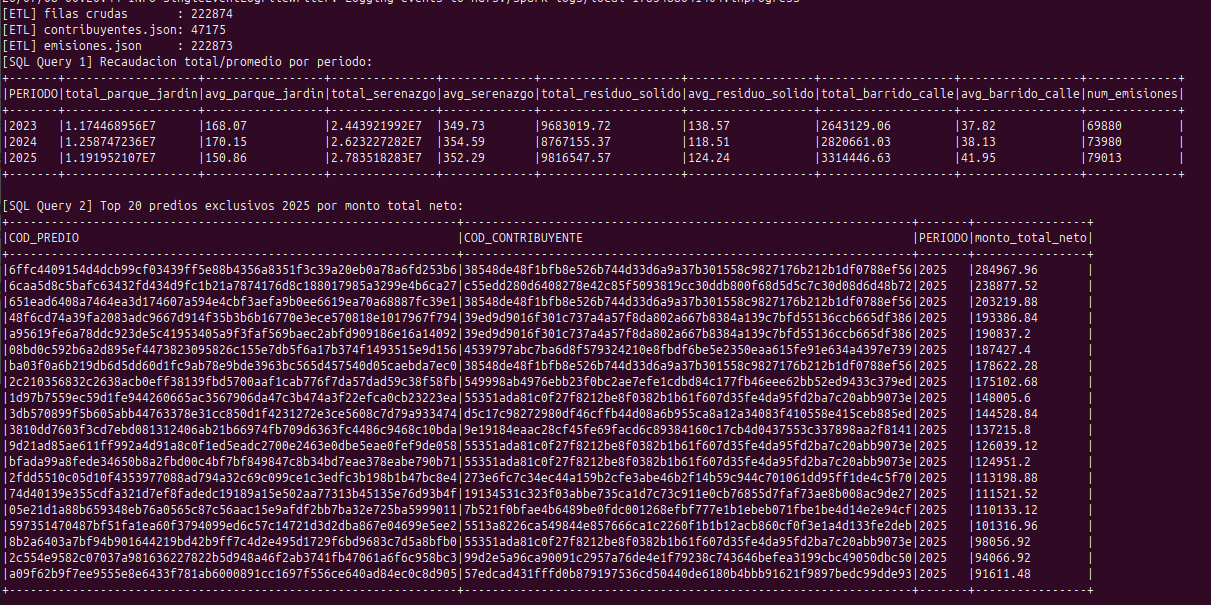
\includegraphics[width=\textwidth]{ImgNod1/ETL_SQL.png}
    \caption{Ejecucion mononodo: conteos ETL y resultados de las dos consultas en terminal.}
    \label{fig:local-etl-sql}
\end{figure}

\section{Modelos Spark ML}

\subsection{Preparacion de variables}

Los modelos se entrenaron sobre \texttt{emisiones.json}. Para regresion se usaron ocho variables explicativas: \texttt{PERIODO}, \texttt{PORCENTAJE\_CONDOMINIO}, montos de parques, residuos y barrido, y descuentos/topes seleccionados. La variable objetivo fue \texttt{MONTO\_SERENAZGO}.

Para clasificacion se construyo la etiqueta \texttt{TIPO\_PREDIO}: \textit{Exclusivo} cuando \texttt{PORCENTAJE\_CONDOMINIO = 100} y \textit{Compartido} en los demas casos. Esta columna no se uso como feature en clasificacion, porque incluirla generaria fuga de datos: el modelo aprenderia directamente el umbral que define la etiqueta.

En ambos casos se aplico division entrenamiento/prueba de 80/20 con semilla fija y normalizacion de variables mediante \texttt{StandardScaler}. Por ello, las metricas no se calculan sobre los mismos registros usados para entrenar, sino sobre una particion de prueba; esto permite hablar de capacidad predictiva bajo condiciones similares a las observadas en el dataset.

\subsection{Regresion}

El enunciado solicita una regresion con Multilayer Perceptron y otra basada en maquinas de soporte vectorial. Spark MLlib no incluye de forma directa un MLP de regresion ni un SVR equivalente para regresion, por lo que ambos fueron derivados manualmente:

\begin{itemize}
    \item \textbf{MLPRegressor}: red con una capa oculta de 16 neuronas, activacion \texttt{tanh}, salida lineal y perdida MSE. El entrenamiento distribuye el calculo del gradiente mediante \texttt{treeAggregate}.
    \item \textbf{SVRegressor}: regresion de soporte vectorial lineal con perdida epsilon-insensitiva y regularizacion L2. Tambien usa agregacion distribuida de subgradientes.
\end{itemize}

\subsection{Clasificacion}

Para clasificacion se utilizaron algoritmos disponibles en Spark MLlib:

\begin{itemize}
    \item \textbf{Random Forest}: 100 arboles y profundidad maxima 8.
    \item \textbf{Multilayer Perceptron Classifier}: arquitectura \texttt{[7, 8, 4, 2]} con 200 iteraciones.
\end{itemize}

\subsection{Curvas de perdida}

Las curvas de perdida se generaron para los dos modelos derivados de regresion, porque en ellos el entrenamiento iterativo se implemento manualmente. Random Forest no expone una curva de perdida por epoca y \texttt{MultilayerPerceptronClassifier} usa optimizacion interna de Spark sin historial exportado equivalente.

\begin{figure}[H]
    \centering
    \begin{subfigure}{0.49\textwidth}
        \centering
        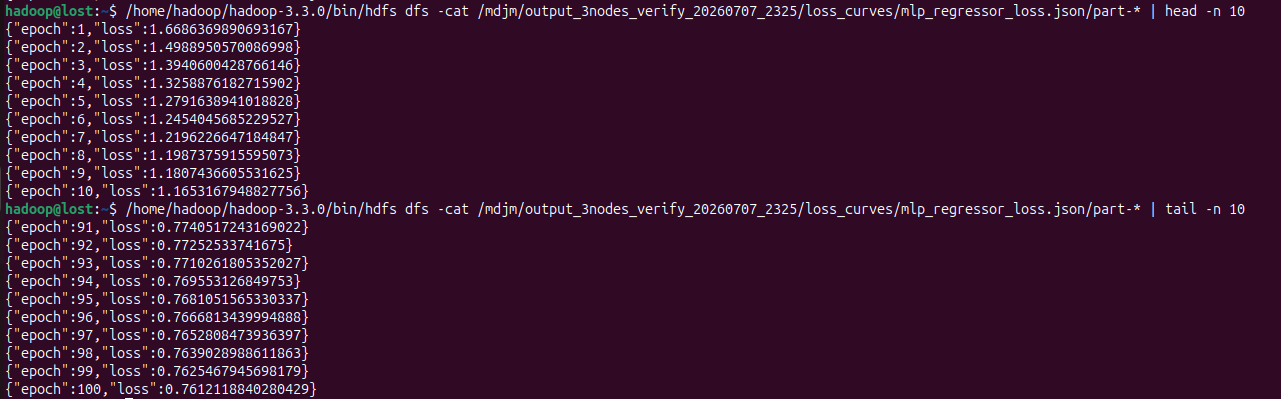
\includegraphics[width=\textwidth]{ImgNod1/Curva_Perdida_MLP_Regre.png}
        \caption{MLPRegressor.}
    \end{subfigure}
    \begin{subfigure}{0.49\textwidth}
        \centering
        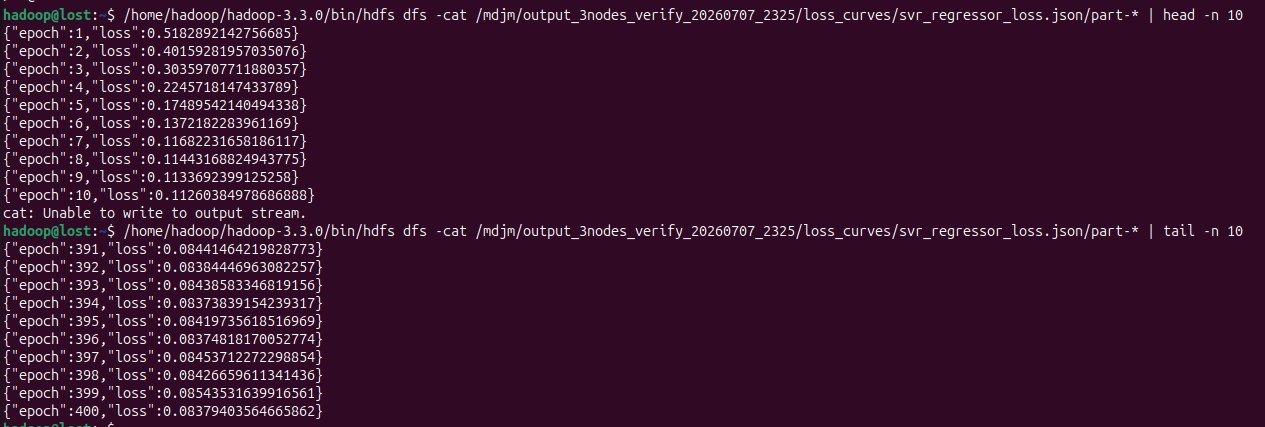
\includegraphics[width=\textwidth]{ImgNod1/Curva_Perdida_svr_regresor.png}
        \caption{SVRegressor.}
    \end{subfigure}
    \caption{Curvas de perdida de entrenamiento para los modelos de regresion derivados.}
    \label{fig:loss-curves}
\end{figure}

\section{Resultados experimentales}

\subsection{Comparacion de rendimiento}

La Tabla~\ref{tab:performance} compara la ejecucion completa del proyecto en un nodo frente a la ejecucion completa en el cluster YARN de tres nodos. Se usa como referencia la ejecucion \texttt{all}, que incluye ETL, consultas SQL, regresion y clasificacion.

\begin{table}[H]
    \centering
    \caption{Comparacion de rendimiento mononodo vs. multimodo.}
    \label{tab:performance}
    \footnotesize
    \renewcommand{\arraystretch}{1.15}
    \begin{tabularx}{\textwidth}{
        >{\raggedright\arraybackslash}p{0.15\textwidth}
        >{\centering\arraybackslash}p{0.07\textwidth}
        >{\centering\arraybackslash}p{0.08\textwidth}
        >{\centering\arraybackslash}p{0.13\textwidth}
        >{\centering\arraybackslash}p{0.13\textwidth}
        >{\centering\arraybackslash}p{0.08\textwidth}
        X}
        \toprule
        \textbf{Ambiente} & \textbf{Nodos} & \textbf{Vcores} & \textbf{Memoria YARN} & \textbf{Tiempo} & \textbf{Speedup} & \textbf{Observacion} \\
        \midrule
        Mononodo local & 1 & 2 aprox. & N/A & 7 min 02.693 s & 1.00 & Ejecucion \texttt{local[*]} sobre archivo local. \\
        Multimodo YARN & 3 & 4 & 8 GB & 18 min 45 s & 0.38 & Ejecucion distribuida sobre HDFS; mayor overhead por YARN, HDFS, shuffle y VMs. \\
        \bottomrule
    \end{tabularx}
\end{table}

\begin{table}[H]
    \centering
    \caption{Asignacion de recursos observada durante una ejecucion distribuida.}
    \label{tab:resources}
    \footnotesize
    \renewcommand{\arraystretch}{1.15}
    \begin{tabularx}{\textwidth}{
        >{\raggedright\arraybackslash}p{0.13\textwidth}
        >{\centering\arraybackslash}p{0.11\textwidth}
        >{\centering\arraybackslash}p{0.10\textwidth}
        >{\centering\arraybackslash}p{0.10\textwidth}
        >{\raggedright\arraybackslash}p{0.17\textwidth}
        >{\raggedright\arraybackslash}p{0.15\textwidth}
        X}
        \toprule
        \textbf{Nodo} & \textbf{Mem. conf.} & \textbf{Vcores conf.} & \textbf{Cont.} & \textbf{Recurso asignado} & \textbf{Uso observado} & \textbf{Rol} \\
        \midrule
        \texttt{master} & 4096 MB & 2 & 2 & 2048 MB, 2 vcores & PMem aprox. 697 MB & Driver/ApplicationMaster y tareas. \\
        \texttt{slave1} & 2048 MB & 1 & 1 & 1024 MB, 1 vcore & PMem aprox. 171 MB & Worker. \\
        \texttt{slave-base} & 2048 MB & 1 & 1 & 1024 MB, 1 vcore & PMem aprox. 176 MB & Worker. \\
        \bottomrule
    \end{tabularx}
\end{table}


\begin{figure}[H]
    \centering
    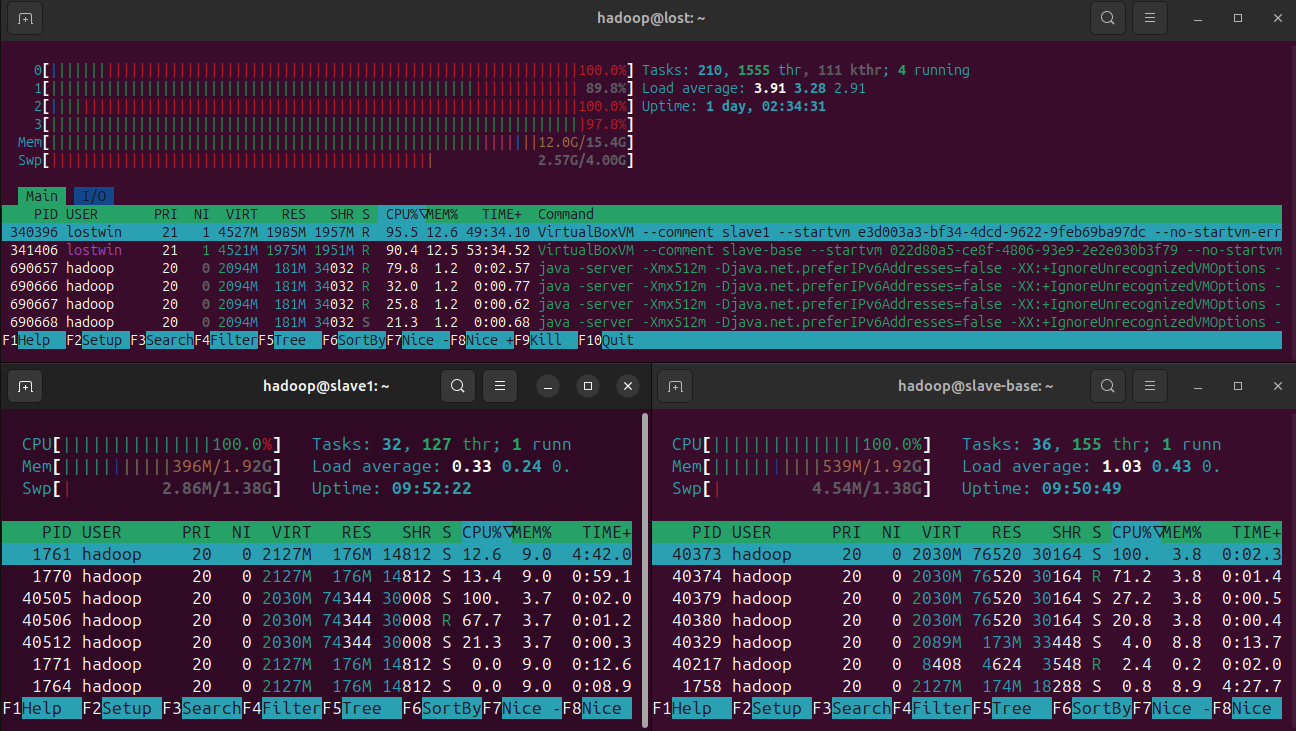
\includegraphics[width=\textwidth]{ImgNod1/Capturas_Rercursos_3nodo_en_vivo.png}
    \caption{Monitor de recursos por nodo durante la ejecucion: master, slave1 y slave-base.}
    \label{fig:htop-all}
\end{figure}

\subsection{Metricas de regresion}

\begin{table}[H]
    \centering
    \caption{Metricas de regresion: comparacion entre mononodo y cluster.}
    \label{tab:regression}
    \begin{tabular}{llrrrr}
        \toprule
        \textbf{Modelo} & \textbf{Ambiente} & \textbf{RMSE} & \textbf{MSE} & \textbf{MAE} & $\boldsymbol{R^2}$ \\
        \midrule
        MLPRegressor & Mononodo & 1352.55 & 1\,829\,399.43 & 281.91 & 0.2233 \\
        MLPRegressor & Cluster & 1384.64 & 1\,917\,232.43 & 284.91 & 0.2302 \\
        SVRegressor & Mononodo & 1430.10 & 2\,045\,182.64 & 232.98 & 0.1317 \\
        SVRegressor & Cluster & 1486.36 & 2\,209\,266.74 & 257.77 & 0.1130 \\
        \bottomrule
    \end{tabular}
\end{table}


En ambos ambientes el MLPRegressor obtuvo mejor RMSE y MSE que el SVRegressor. Los valores de $R^2$ son positivos pero moderados, lo que indica que las variables disponibles explican parte del comportamiento de \texttt{MONTO\_SERENAZGO}, aunque no capturan toda la variabilidad del cobro.

\subsection{Metricas de clasificacion}

\begin{table}[H]
    \centering
    \caption{Metricas de clasificacion: comparacion entre mononodo y cluster.}
    \label{tab:classification}
    \begin{tabular}{llrrrr}
        \toprule
        \textbf{Modelo} & \textbf{Ambiente} & \textbf{Accuracy} & \textbf{Precision} & \textbf{Recall} & \textbf{F1-score} \\
        \midrule
        RandomForest & Mononodo & 0.8614 & 0.8833 & 0.8614 & 0.8421 \\
        RandomForest & Cluster & 0.8593 & 0.8819 & 0.8593 & 0.8397 \\
        MLPClassifier & Mononodo & 0.7458 & 0.8367 & 0.7458 & 0.7615 \\
        MLPClassifier & Cluster & 0.7371 & 0.5433 & 0.7371 & 0.6255 \\
        \bottomrule
    \end{tabular}
\end{table}


Random Forest fue el modelo de clasificacion mas estable y con mejor F1-score. El MLPClassifier alcanzo desempeno superior al azar, pero fue mas sensible al entorno y a la separacion de datos; esto es esperable en una red pequena sin mayor ajuste de hiperparametros.

\begin{figure}[H]
    \centering
    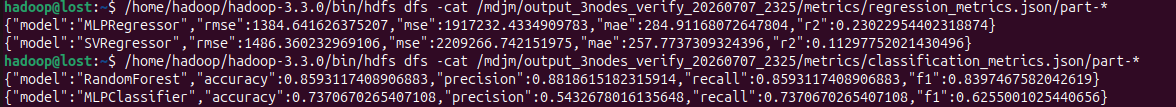
\includegraphics[width=\textwidth]{ImgNod1/Metricas_Regresion_Clasificacion.png}
    \caption{Metricas de regresion y clasificacion obtenidas en la ejecucion multimodo desde HDFS.}
    \label{fig:cluster-metrics-terminal}
\end{figure}

\section{Discusi\'on de resultados}

\subsection{Interpretacion de la comparacion mononodo vs. multimodo}

El cluster distribuido funciono correctamente y ejecuto el proyecto con estado final \texttt{SUCCEEDED}. Sin embargo, para este dataset el entorno mononodo fue mas rapido. La razon principal es que el volumen de datos es pequeno para un cluster: 58 MB en CSV y 222\,874 registros. En ese rango, el costo fijo de iniciar aplicaciones YARN, coordinar contenedores, leer desde HDFS, serializar datos, mover bloques de shuffle y sincronizar resultados puede superar el beneficio de paralelizar.

Tambien influyo el contexto de virtualizacion. Los nodos workers tienen recursos ajustados, especialmente 2 GB de RAM y 1 vcore cada uno. Durante algunas ejecuciones aparecieron advertencias \texttt{FetchFailed}; Spark pudo recuperarse mediante reintentos y la aplicacion finalizo correctamente, pero esos reintentos aumentan el tiempo total. En un dataset mayor, o con workers con mas memoria y CPU, el cluster deberia mostrar mejor escalamiento.

\subsection{Interpretacion de las consultas SQL}

La consulta por periodo muestra que el numero de emisiones aumento de 69\,880 en 2023 a 79\,013 en 2025. Serenazgo es el concepto con mayor monto total en los tres periodos, superando los 24 millones en 2023 y llegando a 27.8 millones en 2025. Barrido de calles tiene el monto total mas bajo, pero crece de 2.64 millones en 2023 a 3.31 millones en 2025.

La consulta de top 20 para 2025 permite identificar predios exclusivos con montos netos excepcionalmente altos. Estos registros son utiles para auditoria, priorizacion de fiscalizacion o analisis de concentracion de la recaudacion.

\subsection{Interpretacion de los modelos}

En regresion, el MLPRegressor logra el menor error global. El SVRegressor tiene menor MAE local, pero mayor RMSE y MSE, lo que sugiere mayor sensibilidad ante errores grandes. Los valores de $R^2$ moderados indican que la variable \texttt{MONTO\_SERENAZGO} depende de factores adicionales que no estan completamente representados en el dataset.

En clasificacion, Random Forest se comporta mejor que el MLPClassifier. Esto es razonable porque los arboles capturan relaciones no lineales y reglas por umbral con menor necesidad de ajuste fino. El MLPClassifier requiere mayor calibracion de arquitectura, iteraciones y posiblemente balanceo de clases para mejorar su F1-score.

\section{Conclusiones}

Se implemento y valido un flujo completo de procesamiento en Spark con HDFS para el dataset de arbitrios municipales de Jesus Maria. El proyecto genero dos tablas JSON, ejecuto dos consultas Spark SQL, entreno dos modelos de regresion y dos modelos de clasificacion, y produjo salidas reproducibles en mononodo y multimodo.

El cluster multimodo demostro paralelismo real: YARN reporto tres nodos activos, contenedores distribuidos y recursos asignados en master y workers. La aplicacion finalizo con estado \texttt{SUCCEEDED}. La comparacion de rendimiento, no obstante, favorecio al mononodo debido al tamano moderado del dataset y al overhead del entorno distribuido.

Desde el punto de vista analitico, la mayor carga de emision corresponde a serenazgo, mientras que Random Forest fue el mejor clasificador de tipo de predio y MLPRegressor fue el mejor regresor para estimar \texttt{MONTO\_SERENAZGO}. Los resultados son consistentes y defendibles para una demostracion en vivo, siempre que se explique que el objetivo del examen es demostrar configuracion, ejecucion distribuida y comparacion, no necesariamente obtener aceleracion con una base pequena.

\section{Referencias}

\begin{thebibliography}{9}

\bibitem{pnda}
Plataforma Nacional de Datos Abiertos del Peru.
\textit{Emision de arbitrios municipales de la Municipalidad Distrital de Jesus Maria}.
Municipalidad Distrital de Jesus Maria - Lima. Fecha de lanzamiento: 2025-04-24. Fecha de modificacion: 2025-08-06. Disponible en: \url{https://www.datosabiertos.gob.pe/dataset/emisi%C3%B3n-de-arbitrios-municipales-de-la-municipalidad-distrital-de-jes%C3%BAs-mar%C3%ADa-mdjm}. Consulta del proyecto: julio de 2026.

\bibitem{spark}
Apache Software Foundation.
\textit{Apache Spark Documentation}.
Disponible en: \url{https://spark.apache.org/docs/latest/}.

\bibitem{hadoop}
Apache Software Foundation.
\textit{Apache Hadoop Documentation}.
Disponible en: \url{https://hadoop.apache.org/docs/}.

\bibitem{yarn}
Apache Software Foundation.
\textit{Apache Hadoop YARN}.
Disponible en: \url{https://hadoop.apache.org/docs/current/hadoop-yarn/hadoop-yarn-site/YARN.html}.

\bibitem{opendata}
OECD.
\textit{Open Government Data}. OECD Digital Government Studies.
Referencia conceptual para el uso de datos abiertos en transparencia y mejora de servicios publicos.

\end{thebibliography}

\appendix
\section{Comandos de ejecuci\'on y rutas}
\label{app:commands}

\subsection{Compilacion}

\begin{lstlisting}[language=bash]
cd /home/lostwin/Documentos/Sublime-Data/2026-I/MACRODATOS/Final-Macrodatos
make build
\end{lstlisting}

\subsection{Ejecucion mononodo}

\begin{lstlisting}[language=bash]
cd /home/lostwin/Documentos/Sublime-Data/2026-I/MACRODATOS/Final-Macrodatos
time make run-all
\end{lstlisting}

Esta ejecucion usa por defecto:

\begin{lstlisting}[language=bash]
SPARK_MASTER=local[*]
INPUT=file:///.../Final-Macrodatos/data/dataset_vf_3.csv
OUTPUT=file:///.../Final-Macrodatos/output
\end{lstlisting}

\subsection{Ejecucion multimodo sobre YARN}

\begin{lstlisting}[language=bash]
/opt/spark/bin/spark-submit \
  --class mdjm.Main \
  --master yarn \
  --conf spark.executor.instances=3 \
  --conf spark.dynamicAllocation.enabled=false \
  --conf spark.executor.cores=1 \
  --conf spark.executor.memory=512m \
  --conf spark.executor.memoryOverhead=384 \
  --conf spark.sql.shuffle.partitions=4 \
  /tmp/arbitrios-mdjm.jar \
  hdfs:///mdjm/input/dataset_vf_3.csv \
  hdfs:///mdjm/output_3nodes_verify_20260707_2325 \
  all
\end{lstlisting}

\subsection{Verificacion de salidas en HDFS}

\begin{lstlisting}[language=bash]
hdfs dfs -ls -R /mdjm/output_3nodes_verify_20260707_2325
hdfs dfs -cat /mdjm/output_3nodes_verify_20260707_2325/metrics/regression_metrics.json/part-*
hdfs dfs -cat /mdjm/output_3nodes_verify_20260707_2325/metrics/classification_metrics.json/part-*
hdfs dfs -cat /mdjm/output_3nodes_verify_20260707_2325/queries/query1_groupby_periodo.json/part-*
hdfs dfs -cat /mdjm/output_3nodes_verify_20260707_2325/queries/query2_top_predios_2025.json/part-* | head
\end{lstlisting}

\subsection{Salidas adjuntas en el proyecto del informe}

Para facilitar la revision en Overleaf, se adjuntan las salidas livianas en la carpeta \texttt{salidas/}:

\begin{itemize}
    \item \texttt{salidas/queries/}: JSON de las dos consultas Spark SQL.
    \item \texttt{salidas/metrics/}: metricas de regresion y clasificacion.
    \item \texttt{salidas/loss\_curves/}: puntos de las curvas de perdida de MLPRegressor y SVRegressor.
\end{itemize}

Las tablas completas \texttt{contribuyentes.json} y \texttt{emisiones.json}, asi como el CSV de entrada, se mantienen como entregables del proyecto por fuera del PDF debido a su mayor tamano.

\section{Capturas complementarias}

\begin{figure}[H]
    \centering
    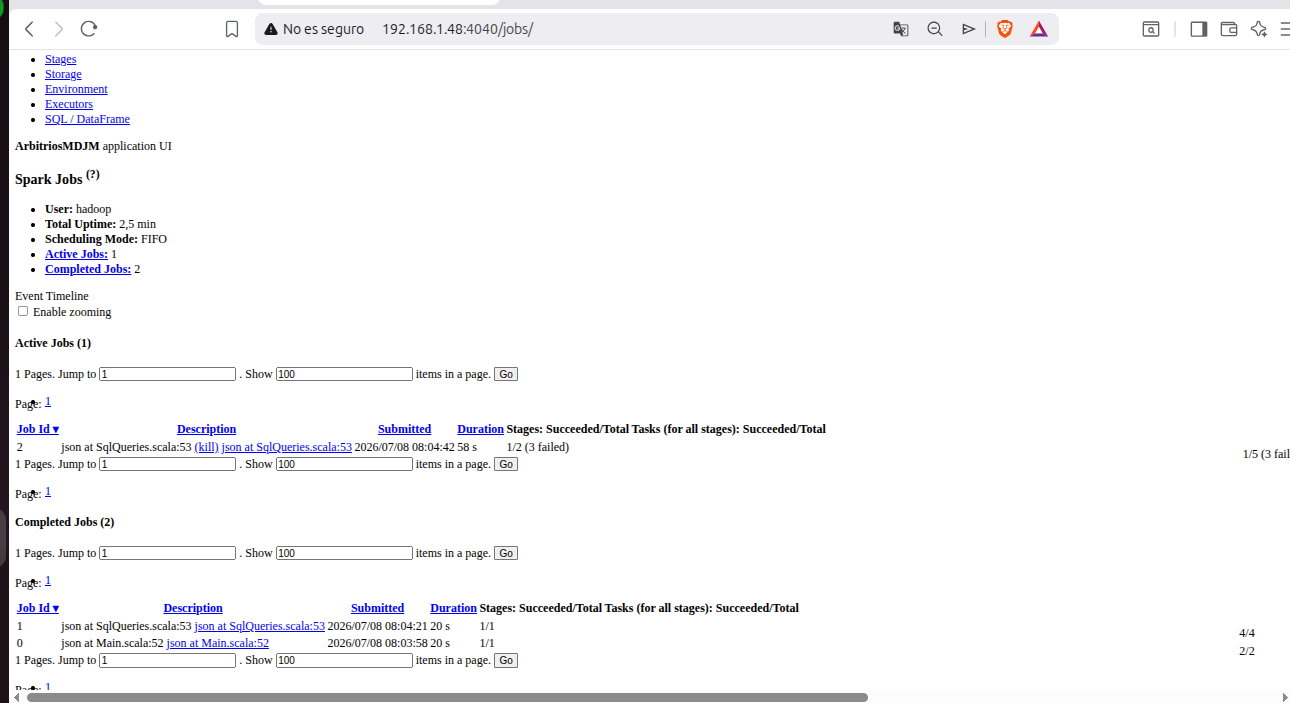
\includegraphics[width=\textwidth]{ImgMultiNodo/SPARKUISQL.png}
    \caption{Spark UI durante la ejecucion de consultas SQL en el cluster.}
    \label{fig:spark-ui-sql}
\end{figure}

\begin{figure}[H]
    \centering
    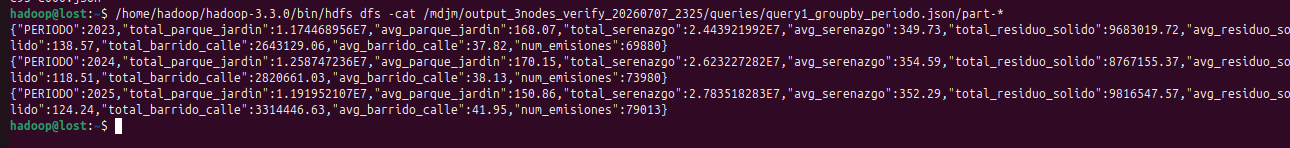
\includegraphics[width=\textwidth]{ImgMultiNodo/Query1_Resultado_Head.png}
    \caption{Salida JSON de la consulta 1 en HDFS.}
    \label{fig:query1-head}
\end{figure}

\begin{figure}[H]
    \centering
    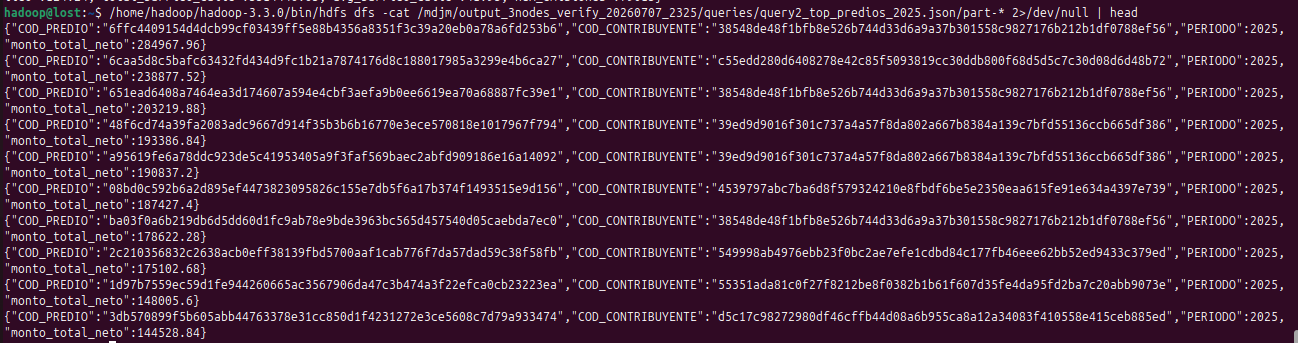
\includegraphics[width=\textwidth]{ImgMultiNodo/Query2_resultado_Head.png}
    \caption{Salida JSON de la consulta 2 en HDFS.}
    \label{fig:query2-head}
\end{figure}

\section{Archivos Scala adjuntos}
\label{app:scala}

Los archivos fuente fueron copiados dentro de este proyecto de informe en la ruta \texttt{codigo/mdjm/}. A continuacion se listan los archivos principales que implementan cada requerimiento:

\begin{itemize}
    \item \texttt{codigo/mdjm/ETL.scala}
    \item \texttt{codigo/mdjm/SqlQueries.scala}
    \item \texttt{codigo/mdjm/FeaturePipeline.scala}
    \item \texttt{codigo/mdjm/Main.scala}
    \item \texttt{codigo/mdjm/MetricsWriter.scala}
    \item \texttt{codigo/mdjm/mlp/MLPRegressor.scala}
    \item \texttt{codigo/mdjm/svr/SVRegressor.scala}
    \item \texttt{codigo/mdjm/classification/RFAndMLPClassification.scala}
\end{itemize}

\subsection{Fragmento ETL}
\lstinputlisting[language=scala,firstline=1,lastline=95]{codigo/mdjm/ETL.scala}

\subsection{Consultas SQL}
\lstinputlisting[language=scala,firstline=1,lastline=65]{codigo/mdjm/SqlQueries.scala}

\subsection{Orquestador principal}
\lstinputlisting[language=scala,firstline=1,lastline=110]{codigo/mdjm/Main.scala}


\end{document}
